\section{总体介绍}

\begin{frame}
    \frametitle{开发情况}

    \begin{itemize}
        \item 内核一共 1.6 万行代码
        \item 实现了 77 条系统调用,能够支持 busybox, UnixBench 等测试
        \item \strong{同一份二进制可同时在多个平台 (QEMU / VisionFive V2) 上启动}
        \item \strong{能够在模拟器上运行 Linux}
    \end{itemize}

\end{frame}

\begin{frame}
    \frametitle{总体架构}
    \begin{figure}
        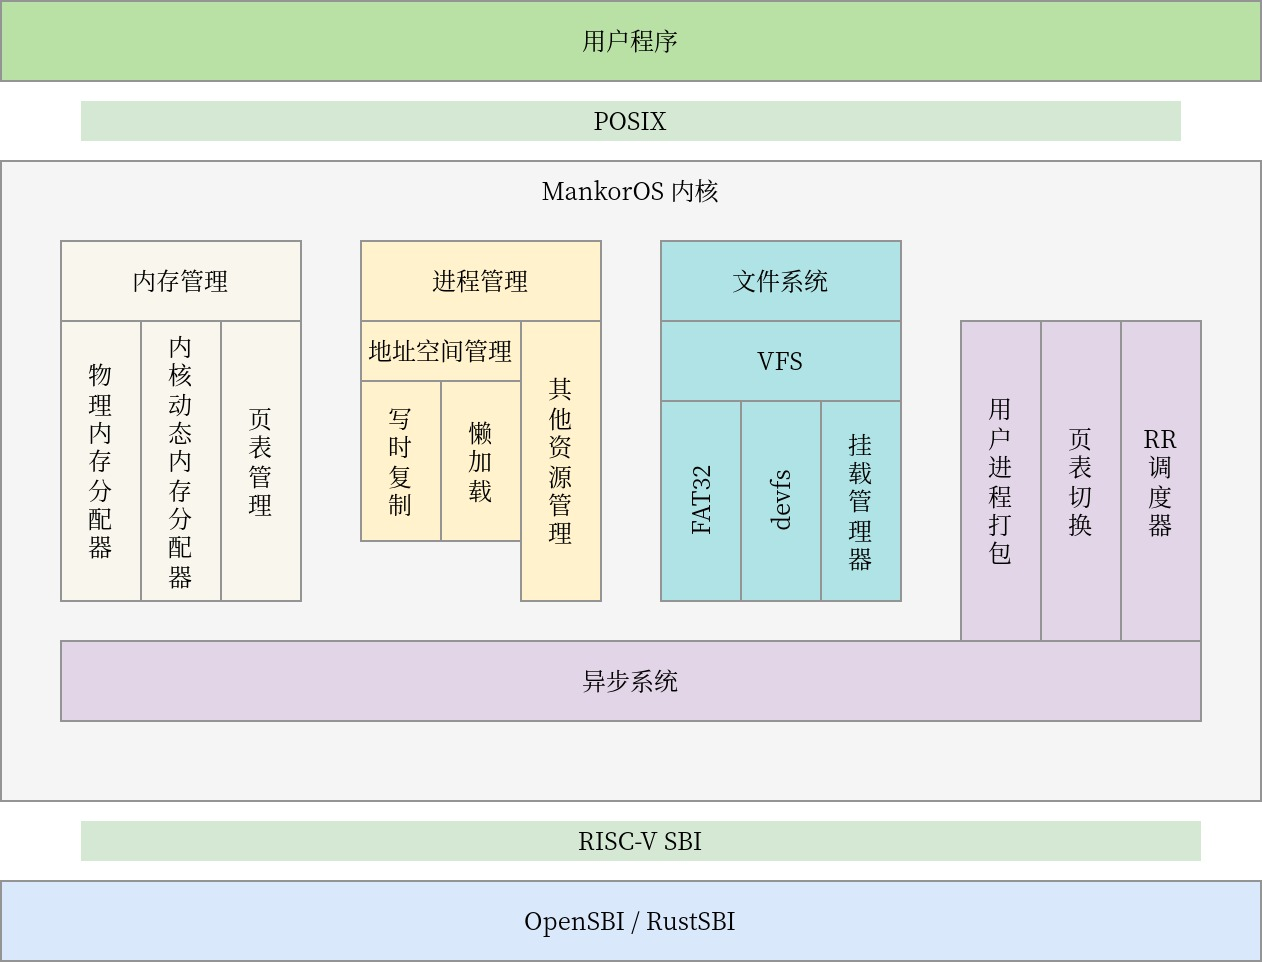
\includegraphics[width=.6\textwidth]{assets/Arch.jpg}
    \end{figure}

\end{frame}

\begin{frame}
    \frametitle{基本优化}
    \begin{columns}
        \begin{column}{.5\linewidth}
            \begin{enumerate}
                \item 进程地址空间
                      \begin{itemize}
                          \item 写时复制 (CoW)
                          \item mmap private 懒加载
                          \item mmap annoymous 懒分配
                      \end{itemize}
                \item ELF 解析
                      \begin{itemize}
                          \item 异步解析
                          \item 复用 mmap private 懒加载
                      \end{itemize}
                \item 物理内存与上下文切换
                      \begin{itemize}
                          \item 共享内核页表
                          \item 按需浮点上下文保存
                          \item 无锁物理页引用计数
                      \end{itemize}
            \end{enumerate}
        \end{column}

        \begin{column}{.5\linewidth}
            \begin{enumerate}
                \setcounter{enumi}{3}
                \item VFS
                      \begin{itemize}
                          \item 页缓存
                          \item 路径缓存
                          \item 文件元信息缓存
                      \end{itemize}
                \item Fat32
                      \begin{itemize}
                          \item (目录内容的) 块缓存
                          \item FAT 缓存
                          \item 文件簇链缓存
                      \end{itemize}
                \item 系统调用
                      \begin{itemize}
                          \item 统一子函数签名以使用跳转表
                          \item 基于特定内核异常捕捉的\\
                                快速用户指针检查
                                %   \item 零拷贝 IO 接口
                      \end{itemize}
            \end{enumerate}
        \end{column}
    \end{columns}
\end{frame}
